\documentclass[letterpaper]{article}
\usepackage[utf8]{inputenc}
%\usepackage[ansinew]{inputenc}
\usepackage[spanish]{babel}
\usepackage{graphicx}

\begin{document}

\title{Proyecto 4\\ Laboratorio de Microcontroladores Motor DC}
\author{
 Marco Antonio Montero Chavarría Carné: A94000\\
  \and
  Francisco Molina Carné: B14194\\  
}
\maketitle

\section{Cambios en la solución propuesta}
Con respecto a la solución propuesta en el anteproyecto no se realizaron muchos cambios, en cuanto al esquema se utilizó la misma línea de desarrollo mostrada en la figura \ref{esque}.  Para lograrlo se siguió el procedimiento de forma que, primero se probó que funcionara el circuito de alimentación del motor y que las tensiones fueran las adecuadas de acuerdo con la figura \ref{circ}, ya que se utilizó una fuente externa para la alimentación del motor, esto para proveer la corriente necesaria en caso de que el motor exigiera más de lo soportado por el microcontrolador. 
\begin{center}
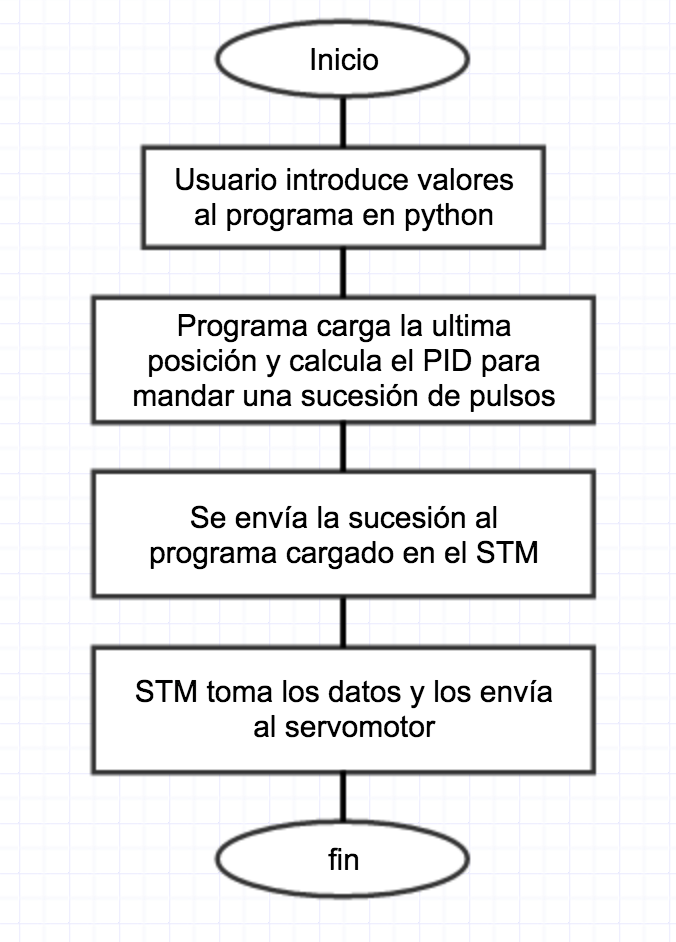
\includegraphics[width=6cm]{micro.png}
\label{esque}
\end{center}
Una vez realizado el circuito se procedió a probar con diferentes ciclos de trabajo para el pwm, variando primero manualmente los valores dentro del programa de C, hasta encontrar un rango que permitiera abarcar los 180 grados de capacidad del motor. 

\begin{center}
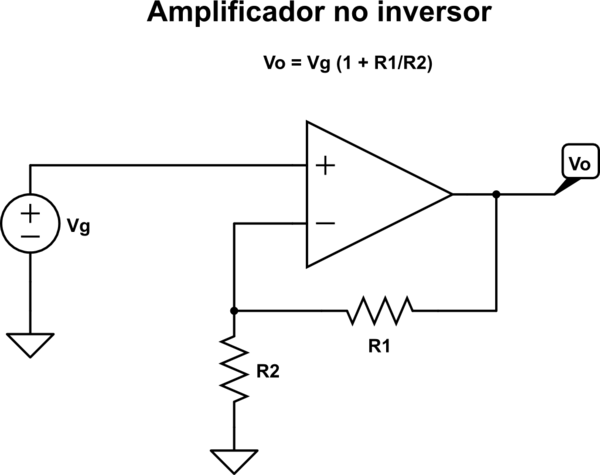
\includegraphics[width=5cm]{amp.png}
\label{circ}
\end{center}

Con el rango definido, se realizó una pequeña multiplicación, dejando variar la posición del motor dependiendo de 1 variable que puede contener valores entre 1 y 8 para cubrir la totalidad del movimiento del servo, esto se realizó a manera de prueba, aunque convencionalmente se utiliza un rango de 0 a 255. Se incluyo además en el codigo que se leyera constantemente en el archivo de C, el puerto serial, de forma que si llega un nuevo valor separado por un "enter", se tomara este como la posición deseada y se cambiara a la misma.
Una vez logrados estos objetivos se procedió a elaborar el control de velocidad, en el cual se incluyó en el programa de python un campo para definir la velocidad a la que se quería cambiar. El control de velocidad funciona de forma que toma el ángulo actual, el ángulo objetivo y recibe como entrada la cantidad de divisiones que quiere llevar a cabo entre estos 2, y ejecuta una por una las divisiones con cierto tiempo de separación para lograr un movimiento suave. 

 
\newpage

\section{Innovación}
A manera de innovación se pensó realizar un control en el cambio de velocidad que no fuera precisamente lineal, si no que cambiara proporcinalmente a la posición deseada, esto pensando en por ejemplo el control de una motocicleta, que debar tener un arranque suave para no tener ningún accidente con el torque de arranque. Sin embargo para el proyecto se realizó el inverso, lo que tendria aplicaciones en funciones donde se ocupe una cierta precisión en la llegada del motor. De esta forma al subdividir la posición deseada, con cada paso lo que se hizo fue disminuir la partición a la mitad con cada una de las realizadas, de forma que la velocidad dismuya conforme se acerca al angulo deseado, como se muestra en el video: \\
https://youtu.be/0XwXEmdkR04
.

\newpage
\section{Justificación de resultados}
Aspectos como respetar el diagrama del circuito y realizar el proyecto estructuradamente de forma que se probara siempre antes de realizar cualquier paso, fueron fundamentales para llevar a cabo la tarea sin ningún inconveniente mayor. Cerciorarse de las señales y aspectos como la tensión y el ciclo de trabajo de las mismas, permitieron visualizar de mejor forma lo que se está enviando al motor y como este reacciona ante las mismas.\\
Asímismo es de gran ayuda tener como referencia los trabajos anteriores, ya que se comprende de mejor forma el funcionamiento de otras partes del proyecto como la comunicación serial y la temporización de atención a interrupciones del microcontrolador, que fueron necesarias para lograr el panel de control en tiempo real del motor.
\\
En cuanto a la innovación, se prueba con la funcionalidad de no solo variar la posición si no tambien variar la velocidad de movimiento de una forma proporcional, esto aclara y lleva un poco mas allá el manejo de las herramientas, lo que podría llegar a utilizarse en diferentes aplicaciones de una mejor forma, logrando sistemas de control mas eficientes.
\newpage
\section{Recomendaciones}
\begin{itemize}
\item Estructurar el proyecto y probar cada paso antes de realizarlo.
\item Cerciorarse de las señales que se tienen en la salida de cada cable importante.
\item Definir un protocolo para la comunicación serial, que ambos tengan el mismo sistema.
\item Pensar en aplicaciones para los servos y desarrollar en base a esas aplicaciones el aspecto de innovación
\end{itemize}

\bibliographystyle{alpha} 
\bibliography{refs}



\end{document}
